% =====================================================================
%  FedPEFT-IMU - manuscript (IEEE journal format: IoT-J / JBHI / TMC)
%
%  Build:   pdflatex main && bibtex main && pdflatex main && pdflatex main
%  Numbers in the dataset section are generated by
%           python scripts/tools/paper_dataset_stats.py   (-> generated/*.tex)
%  Sections written so far: III (proposed method) and IV (dataset & protocol).
% =====================================================================
% Minimal TeX installations may lack grfext (needed only for EPS conversion; all
% figures here are PDF/TikZ): skip epstopdf in that case via pdftex.def's hook.
\IfFileExists{grfext.sty}{}{\def\DoNotLoadEpstopdf{}}
\documentclass[journal]{IEEEtran}

% ---------------------------------------------------------------- packages
\usepackage{amsmath,amssymb,amsfonts}
\usepackage{mathtools}
\usepackage{bm}
\usepackage[ruled,vlined,linesnumbered]{algorithm2e}
\usepackage{graphicx}
\usepackage{array,tabularx,multirow,makecell,threeparttable}
\newcolumntype{Y}{>{\raggedright\arraybackslash}X}   % ragged-right X column
\usepackage[table]{xcolor}
\usepackage{siunitx}
\usepackage{pifont}
\usepackage{cite}
\usepackage{url}
\usepackage{balance}
\usepackage{microtype}
\usepackage{enumitem}
\usepackage{tikz}
\usetikzlibrary{arrows.meta,positioning,fit,backgrounds,shadows,calc,shapes.geometric,decorations.pathreplacing}
% booktabs is used when installed; otherwise rules fall back to plain lines.
\IfFileExists{booktabs.sty}{\usepackage{booktabs}}{%
  \newcommand{\toprule}{\hline\hline}\newcommand{\midrule}{\hline}\newcommand{\bottomrule}{\hline\hline}}
% hyperref is skipped on minimal local TeX installations that lack its helper
% packages (the document is identical apart from clickable links).
\IfFileExists{bigintcalc.sty}{\usepackage[hidelinks]{hyperref}}{}
\usepackage[capitalize,nameinlink]{cleveref}

% ---------------------------------------------------------------- colours (Okabe-Ito)
\definecolor{cFed}{HTML}{0072B2}     % federated / shared
\definecolor{cLoc}{HTML}{009E73}     % local / private
\definecolor{cStat}{HTML}{E69F00}    % statistics
\definecolor{cFrozen}{HTML}{8C8C8C}  % frozen

% ---------------------------------------------------------------- theorem-like
\newtheorem{proposition}{Proposition}
\newtheorem{lemma}{Lemma}
\newtheorem{remark}{Remark}
\newtheorem{corollary}{Corollary}
\crefname{proposition}{Proposition}{Propositions}
\crefname{lemma}{Lemma}{Lemmas}
\crefname{remark}{Remark}{Remarks}
\crefname{corollary}{Corollary}{Corollaries}
\crefname{algocf}{Algorithm}{Algorithms}
\crefname{equation}{Eq.}{Eqs.}

% ---------------------------------------------------------------- notation
\newcommand{\R}{\mathbb{R}}
\newcommand{\E}{\mathbb{E}}
\newcommand{\Dk}{\mathcal{D}_k}
\newcommand{\St}{\mathcal{S}_t}
\newcommand{\Lset}{\mathcal{L}}
\newcommand{\ptil}{\tilde{p}}
\newcommand{\Wbar}{\bar{W}}
\newcommand{\rmax}{r_{\max}}
\newcommand{\CE}{\mathrm{CE}}
\newcommand{\norm}[1]{\lVert #1\rVert}
\newcommand{\nrm}[1]{\bar{#1}}              % l2-normalised vector
\newcommand{\trunc}[2]{#1_{[#2]}}           % first #2 rank-1 components of a factor
\newcommand{\method}{FedPEFT-IMU}
\newcommand{\NumClients}{106}
\newcommand{\NumHeldout}{30}
\newcommand{\NumPool}{15}
\newcommand{\NumClasses}{6}
% Generated by scripts/tools/paper_dataset_stats.py - do not edit by hand.
\newcommand{\NWindowsFull}{921{,}656}
\newcommand{\NHoursFull}{2{,}560}
\newcommand{\HoursPerUserMedian}{17.1}
\newcommand{\HoursPerUserMin}{6.1}
\newcommand{\HoursPerUserMax}{24.7}
\newcommand{\ImbalanceRatio}{40}
\newcommand{\PctSleep}{36.9}
\newcommand{\PctSitStand}{39.0}
\newcommand{\PctBicycling}{1.0}
\newcommand{\PctVehicle}{3.8}
\newcommand{\UsersBicycling}{42}
\newcommand{\NWindowsExp}{153{,}672}
\newcommand{\NTrainWindows}{85{,}878}
\newcommand{\NTestWindows}{21{,}518}
\newcommand{\NHeldoutTest}{15{,}237}
\newcommand{\NPoolWindows}{15{,}816}
\newcommand{\ClientsBicyclingPct}{26}
\newcommand{\ClientsVehiclePct}{58}
\newcommand{\ClassesPerClient}{4.82}
\newcommand{\AllSixPct}{8}
\newcommand{\JSDMean}{0.065}
\newcommand{\JSDMax}{0.387}
\newcommand{\JSDTrainTest}{0.226}
\newcommand{\DirAlpha}{1.79}
\newcommand{\UnseenClientsPct}{3}
\newcommand{\UnseenWindowsPct}{1.2}
\newcommand{\WinPerClientMedian}{816}
\newcommand{\WinPerClientMin}{302}
\newcommand{\WinPerClientMax}{1156}
\newcommand{\GiniClients}{0.09}
\newcommand{\SelfTransMin}{0.77}
\newcommand{\SelfTransMax}{1.00}
\newcommand{\SleepTrainPct}{30}
\newcommand{\SleepTestPct}{60}
\newcommand{\TestMostlySleepPct}{57}

% Table rows generated by the statistics script are read with the expandable TeX
% primitive, so that a rule (\bottomrule) may follow them inside a tabular.
\makeatletter
\newcommand{\inputrows}[1]{\@@input #1 }
\makeatother

\begin{document}

\title{\method: Federated Parameter-Efficient Adaptation of Pretrained IMU Encoders
for Human Activity Recognition under Device and Data Heterogeneity}

\author{%
  First~Author,~\IEEEmembership{Student Member,~IEEE},
  Second~Author,~\IEEEmembership{Member,~IEEE}%
  \thanks{Manuscript draft. Code, user partitions and all generated statistics are released with the paper.}%
}

\markboth{IEEE Internet of Things Journal (draft)}{\method}

\maketitle

\begin{abstract}
% TODO: write after the results section is final (about 200 words).
Abstract to be written once the results section is final.
\end{abstract}

\begin{IEEEkeywords}
Federated learning, human activity recognition, inertial sensors, low-rank adaptation,
parameter-efficient fine-tuning, foundation models, personalization, heterogeneity.
\end{IEEEkeywords}

% =====================================================================
\section{Introduction}\label{sec:intro}
% TODO
\textit{[Introduction: to be written.]}

\section{Related Work}\label{sec:related}
% TODO: federated HAR; PEFT/LoRA in FL (FedEx-LoRA, HetLoRA, FLoRA, FlexLoRA, FFA-LoRA);
%       personalised FL (FedBN, FedPer, FedRep, FedProto); IMU foundation models;
%       label skew in FL (FedLC, FedRS, CReFF).
\textit{[Related work: to be written.]}

% =====================================================================
% =====================================================================
%  Section III - Proposed method: FedPEFT-IMU
%  Every equation below corresponds one-to-one to the released code:
%    client model ........ fedpeft/models/{client_model,components,lora}.py
%    aggregation ......... fedpeft/federated/{aggregation,server}.py
%    round loop .......... fedpeft/federated/simulation.py
%    decoding / new users  fedpeft/training/{imbalance,hmm,decoding,heldout}.py
% =====================================================================
\section{Proposed Method: \method}\label{sec:method}

This section formalizes the learning problem (\cref{sec:method:problem}), presents the
architecture and the role assigned to every parameter (\cref{sec:method:arch,sec:method:client}),
derives the client objective (\cref{sec:method:objective}) and the server aggregation rules
together with their exactness guarantees (\cref{sec:method:agg,sec:method:stats}), explains how
label skew is handled (\cref{sec:method:skew}), and describes inference for enrolled and new
users (\cref{sec:method:inference}). The complete procedure is summarized in \cref{alg:fedpeft},
and its cost is analyzed in \cref{sec:method:cost}. \Cref{tab:notation} lists the main notation.

\begin{table}[!t]
\centering
\caption{Main notation.}
\label{tab:notation}
\footnotesize
\renewcommand{\arraystretch}{1.08}
\begin{tabularx}{\columnwidth}{@{}l Y@{}}
\toprule
Symbol & Meaning \\
\midrule
$K$, $\St$, $\rho$ & number of clients, clients selected in round $t$, participation rate \\
$\Dk^{\mathrm{tr}}$, $\Dk^{\mathrm{te}}$ & chronological training / test part of client $k$ \\
$n_k$, $n_{k,c}$ & training windows of client $k$ (in total / of class $c$) \\
$C$, $\boldsymbol{\pi}_k$, $\boldsymbol{\pi}$ & classes, label prior of client $k$, global label prior \\
$\Pi_E$, $a_k$ & fixed preprocessor of encoder $E$, local input adapter \\
$\Wbar_\ell$, $\Lset$ & frozen base weight of adapted layer $\ell$, set of adapted layers \\
$B_\ell$, $A_\ell$, $r_k$, $s$ & LoRA factors, LoRA rank of client $k$, scaling $s=\alpha/r$ \\
$\psi_k$ & local normalization parameters and statistics \\
$g_\theta$, $h_k$ & shared projection head, personal classifier \\
$\mathbf{z}$, $\mathbf{e}$, $\nrm{\mathbf{e}}$ & encoder feature, embedding ($D=64$), $\mathbf{e}/\norm{\mathbf{e}}_2$ \\
$\mathbf{p}_{k,c}$, $\mathbf{P}_c$ & local and global prototype of class $c$ \\
$\ptil_k$ & aggregation weight $n_k/\sum_{j\in\St}n_j$ \\
$\trunc{B}{r}$, $\trunc{A}{r}$ & first $r$ columns of $B$ / first $r$ rows of $A$ \\
$\Delta_{k,\ell}$ & change of client $k$'s LoRA product in one round \\
$N_k$, $\Gamma$ & $C\times C$ transition counts of client $k$, HMM transition matrix \\
\bottomrule
\end{tabularx}
\end{table}

% ---------------------------------------------------------------------
\subsection{Problem Setting and Design Goals}\label{sec:method:problem}

We consider $K$ users, each holding one device with an inertial measurement unit (IMU), e.g., a
smartphone. The device records multi-axis signals (acceleration and, where available, angular
velocity and magnetic field), segmented into windows $\mathbf{x}\in\R^{C\times L}$ (on HARBox $C=9$
axes, $2$\,s at $50$\,Hz, $L=100$) with activity labels $y\in\{1,\dots,C_y\}$; for readability we
write $C$ for the number of activity classes from here on. This gives a chronologically ordered dataset
$\Dk=\{(\mathbf{x}_{k,i},y_{k,i})\}_{i=1}^{|\Dk|}$. Raw windows never leave the device. A
server orchestrates training over rounds $t=0,\dots,T-1$ in which a random subset
$\St$ of $\lceil\rho K\rfloor$ clients participates.

The setting combines four kinds of heterogeneity that, together, distinguish federated human
activity recognition (HAR) from the image and text benchmarks on which most federated
parameter-efficient fine-tuning (PEFT) methods were developed:
\begin{enumerate}[label=(H\arabic*)]
  \item \emph{Label skew}: $\boldsymbol{\pi}_k\neq\boldsymbol{\pi}$; users perform different
        activities, and different amounts of them.
  \item \emph{Feature shift}: $p_k(\mathbf{x}\mid y)$ differs across users because of device
        model, grip and orientation, body size and movement style; on HARBox this is the
        dominant heterogeneity (\cref{sec:data:hetero}).
  \item \emph{System heterogeneity}: devices differ in memory and compute; we model this by a
        per-device budget expressed as a LoRA rank $r_k\in\mathcal{R}=\{2,4,8\}$.
  \item \emph{Temporal dependence}: activities last longer than a window, so consecutive
        windows are correlated; with overlapping windows they even share samples, which an
        evaluation protocol must respect (\cref{sec:data:splits}).
\end{enumerate}
A pretrained IMU encoder $E$ with weights $\Omega_0$, obtained from data outside the
federation, is available to every participant. The design goals are
(G1)~high macro-F1 for \emph{enrolled} users on their \emph{future} data;
(G2)~useful predictions for \emph{new} users with zero or a few labelled windows;
(G3)~low uplink traffic;
(G4)~training within each device's budget $r_k$; and
(G5)~fairness, i.e., a high F1 for the worst-served users.

We cast the problem as personalized federated learning with shared parameters $\Theta$ and
client-specific parameters $\phi_k$:
\begin{equation}\label{eq:global}
  \min_{\Theta}\ \sum_{k=1}^{K} p_k\,\min_{\phi_k}\,F_k(\Theta,\phi_k),\qquad
  p_k=\frac{n_k}{\sum_{j}n_j},
\end{equation}
where $F_k$ is the local objective defined in \cref{sec:method:objective} and $n_k=|\Dk^{\mathrm{tr}}|$.

% ---------------------------------------------------------------------
\subsection{Architecture Overview and Parameter Roles}\label{sec:method:arch}

\begin{figure*}[!t]
  \centering
  \resizebox{\textwidth}{!}{% =====================================================================
%  Fig. 1 - FedPEFT-IMU system architecture (TikZ, vector).
%  Colour code (same as the project report):
%    grey   = frozen pretrained weights        blue   = federated (shared) parameters
%    green  = local / private parameters       amber  = statistics sent to the server
%    dashed = fixed operation without parameters
%  Included by main.tex inside a figure* environment.
% =====================================================================
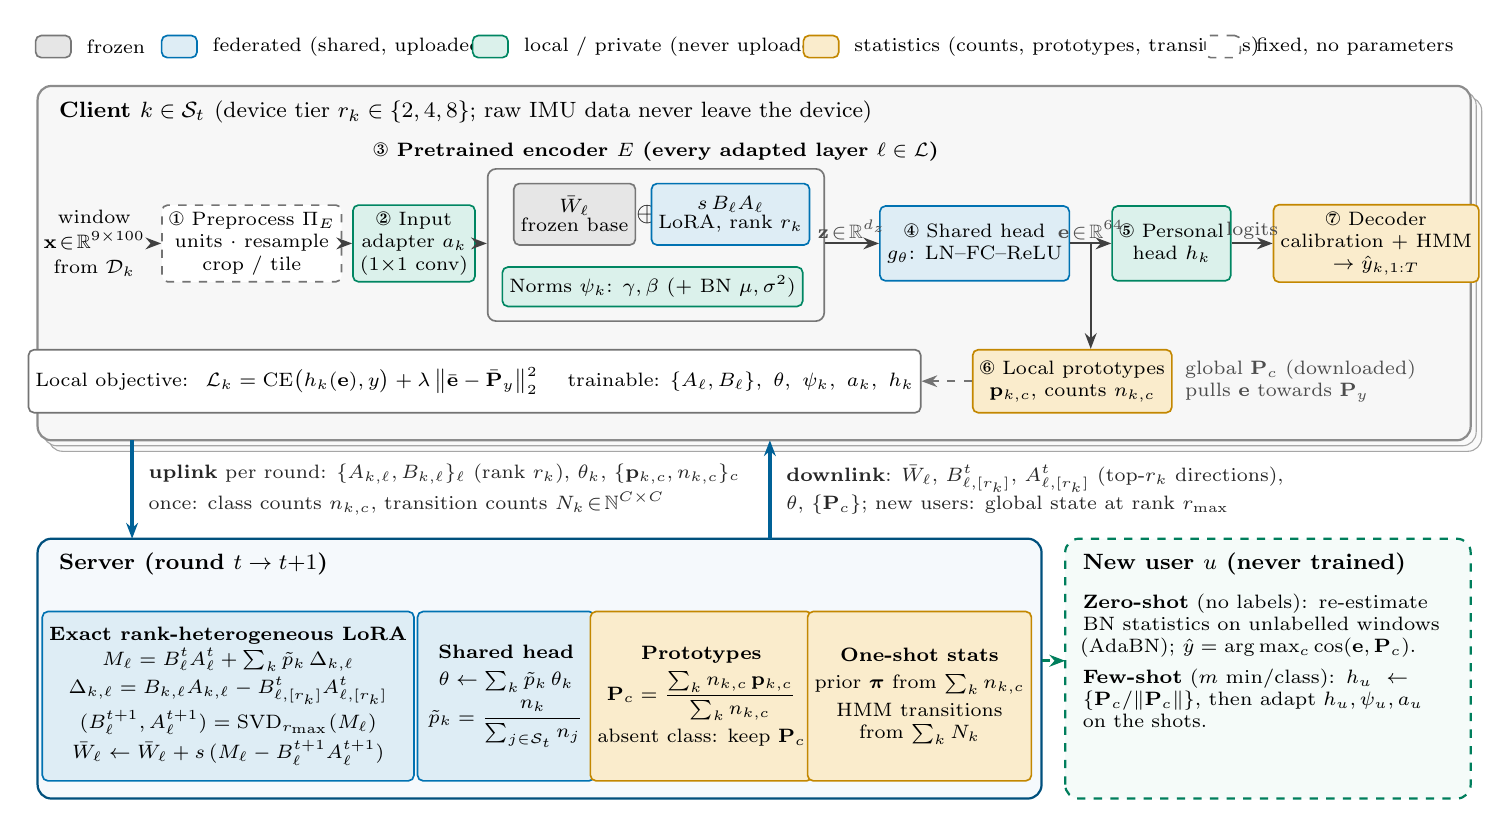
\begin{tikzpicture}[
    font=\scriptsize, >={Stealth[length=2.0mm]},
    blk/.style={rounded corners=2pt, align=center, inner sep=2.5pt, minimum height=0.95cm, line width=0.6pt},
    frozen/.style={blk, fill=cFrozen!22, draw=cFrozen!85!black},
    fed/.style={blk, fill=cFed!13, draw=cFed},
    loc/.style={blk, fill=cLoc!14, draw=cLoc!85!black},
    stat/.style={blk, fill=cStat!20, draw=cStat!85!black},
    fixed/.style={blk, fill=white, draw=black!55, dashed},
    flow/.style={->, line width=0.7pt, draw=black!75},
    lbl/.style={font=\tiny, text=black!70, inner sep=1pt},
    panel/.style={rounded corners=5pt, line width=0.8pt},
  ]

  % ------------------------------------------------------------------ client panel
  % (on the background layer, so that the encoder box drawn later sits on top of it)
  \begin{scope}[on background layer]
    \fill[panel, fill=black!3, draw=black!45, double copy shadow={shadow xshift=0.7mm, shadow yshift=-0.7mm, draw=black!35, fill=black!2}]
         (0,4.55) rectangle (18.2,9.05);
  \end{scope}
  \node[anchor=north west, font=\footnotesize\bfseries] at (0.15,8.98)
       {Client $k\in\mathcal{S}_t$ \textnormal{(device tier $r_k\in\{2,4,8\}$; raw IMU data never leave the device)}};

  % -- data: one window of the local stream (never leaves the device); HARBox: 9 axes x 2 s at 50 Hz
  \node[align=center, font=\scriptsize] (data) at (0.72,7.05)
        {window\\[1pt] $\mathbf{x}\!\in\!\mathbb{R}^{9\times100}$\\[1pt] from $\mathcal{D}_k$};
  % -- (1) preprocessor
  \node[fixed, minimum width=1.85cm] (pre) at (2.72,7.05)
        {\ding{172} Preprocess $\Pi_E$\\ units $\cdot$ resample\\ crop / tile};
  % -- (2) input adapter
  \node[loc, minimum width=1.45cm] (adp) at (4.78,7.05) {\ding{173} Input\\ adapter $a_k$\\ ($1{\times}1$ conv)};

  % -- (3) encoder: frozen base + LoRA + local norms
  \node[frozen, minimum width=1.35cm, minimum height=0.78cm] (wbar) at (6.82,7.42) {$\bar{W}_\ell$\\[-1pt] frozen base};
  \node[font=\normalsize] (plus) at (7.74,7.42) {$\oplus$};
  \node[fed, minimum width=1.6cm, minimum height=0.78cm] (lora) at (8.8,7.42) {$s\,B_\ell A_\ell$\\[-1pt] LoRA, rank $r_k$};
  \node[loc, minimum width=3.47cm, minimum height=0.5cm] (norm) at (7.81,6.5)
        {Norms $\psi_k$: $\gamma,\beta$ (+ BN $\mu,\sigma^2$)};
  \begin{scope}[on background layer]
    \node[rounded corners=3pt, draw=cFrozen!85!black, fill=cFrozen!7, line width=0.6pt, inner sep=5pt,
          fit=(wbar)(lora)(norm), label={[font=\scriptsize\bfseries, yshift=-1pt]above:\ding{174} Pretrained encoder $E$ (every adapted layer $\ell\in\mathcal{L}$)}] (enc) {};
  \end{scope}

  % -- (4) shared head, (5) personal head, (7) decoder (+ output)
  \node[fed, minimum width=1.75cm] (g) at (11.9,7.05) {\ding{175} Shared head\\ $g_\theta$: LN--FC--ReLU};
  \node[loc, minimum width=1.3cm] (h) at (14.4,7.05) {\ding{176} Personal\\ head $h_k$};
  \node[stat, minimum width=2.15cm] (dec) at (17.0,7.05) {\ding{178} Decoder\\ calibration + HMM\\ $\rightarrow\hat{y}_{k,1:T}$};

  \draw[flow] (data) -- (pre);
  \draw[flow] (pre) -- (adp);
  \draw[flow] (adp) -- (enc.west |- adp);
  \draw[flow] (enc.east |- g) -- node[lbl, above, font=\scriptsize]{$\mathbf{z}\!\in\!\mathbb{R}^{d_z}$} (g);
  \draw[flow] (g) -- node[lbl, above, font=\scriptsize](emb){$\mathbf{e}\!\in\!\mathbb{R}^{64}$} (h);
  \draw[flow] (h) -- node[lbl, above, font=\scriptsize]{logits} (dec);

  % -- (6) prototypes and local objective
  \node[stat, minimum width=2.3cm, minimum height=0.8cm] (proto) at (13.14,5.3)
        {\ding{177} Local prototypes\\ $\mathbf{p}_{k,c}$, counts $n_{k,c}$};
  \draw[flow] ($(g.east)!0.5!(h.west)$) -- (proto.north -| {$(g.east)!0.5!(h.west)$});
  \node[blk, draw=black!55, fill=white, minimum width=8.3cm, minimum height=0.8cm] (loss) at (5.55,5.3)
        {Local objective: \ $\mathcal{L}_k=\mathrm{CE}\big(h_k(\mathbf{e}),y\big)+\lambda\,\big\lVert\bar{\mathbf{e}}-\bar{\mathbf{P}}_{y}\big\rVert_2^2$
         \quad trainable: $\{A_\ell,B_\ell\},\ \theta,\ \psi_k,\ a_k,\ h_k$};
  \node[anchor=west, align=left, font=\scriptsize, text=black!70] at (14.45,5.3)
        {global $\mathbf{P}_c$ (downloaded)\\ pulls $\mathbf{e}$ towards $\mathbf{P}_y$};
  \draw[->, dashed, draw=black!55, line width=0.6pt] (proto.west) -- (loss.east);

  % ------------------------------------------------------------------ server panel
  \fill[panel, fill=cFed!4, draw=cFed!70!black] (0,0) rectangle (12.75,3.3);
  \node[anchor=north west, font=\footnotesize\bfseries] at (0.15,3.24) {Server (round $t\rightarrow t{+}1$)};

  \node[fed, minimum width=4.25cm, minimum height=2.15cm] (s1) at (2.42,1.3)
        {\textbf{Exact rank-heterogeneous LoRA}\\[1pt]
         $M_\ell=B_\ell^{t}A_\ell^{t}+\sum_{k}\tilde{p}_k\,\Delta_{k,\ell}$\\[1pt]
         $\Delta_{k,\ell}=B_{k,\ell}A_{k,\ell}-B^{t}_{\ell,[r_k]}A^{t}_{\ell,[r_k]}$\\[1pt]
         $(B^{t+1}_\ell,A^{t+1}_\ell)=\mathrm{SVD}_{r_{\max}}(M_\ell)$\\[1pt]
         $\bar{W}_\ell\leftarrow\bar{W}_\ell+s\,(M_\ell-B^{t+1}_\ell A^{t+1}_\ell)$};
  \node[fed, minimum width=2.25cm, minimum height=2.15cm] (s2) at (5.95,1.3)
        {\textbf{Shared head}\\[2pt] $\theta\leftarrow\sum_{k}\tilde{p}_k\,\theta_k$\\[2pt] $\tilde{p}_k=\dfrac{n_k}{\sum_{j\in\mathcal{S}_t}n_j}$};
  \node[stat, minimum width=2.45cm, minimum height=2.15cm] (s3) at (8.43,1.3)
        {\textbf{Prototypes}\\[2pt] $\mathbf{P}_c=\dfrac{\sum_k n_{k,c}\,\mathbf{p}_{k,c}}{\sum_k n_{k,c}}$\\[2pt] absent class: keep $\mathbf{P}_c$};
  \node[stat, minimum width=2.15cm, minimum height=2.15cm] (s4) at (11.2,1.3)
        {\textbf{One-shot stats}\\[2pt] prior $\boldsymbol{\pi}$ from $\sum_k n_{k,c}$\\[2pt] HMM transitions\\ from $\sum_k N_k$};

  % ------------------------------------------------------------------ new-user panel
  \draw[panel, dashed, draw=cLoc!80!black, fill=cLoc!4] (13.05,0) rectangle (18.2,3.3);
  \node[anchor=north west, font=\footnotesize\bfseries] at (13.15,3.24) {New user $u$ (never trained)};
  \node[anchor=north west, align=left, text width=4.85cm, font=\scriptsize] at (13.15,2.72)
        {\textbf{Zero-shot} (no labels): re-estimate BN statistics on unlabelled windows (AdaBN);
         $\hat{y}=\arg\max_c\cos(\mathbf{e},\mathbf{P}_c)$.\\[3pt]
         \textbf{Few-shot} ($m$ min/class): $h_u\leftarrow\{\mathbf{P}_c/\lVert\mathbf{P}_c\rVert\}$,
         then adapt $h_u,\psi_u,a_u$ on the shots.};

  % ------------------------------------------------------------------ communication
  \draw[->, line width=1.3pt, draw=cFed!85!black] (1.2,4.55) -- (1.2,3.3)
       node[midway, right, align=left, font=\scriptsize, text=black!85, xshift=2pt]
       {\textbf{uplink} per round: $\{A_{k,\ell},B_{k,\ell}\}_\ell$ (rank $r_k$), $\theta_k$, $\{\mathbf{p}_{k,c},n_{k,c}\}_c$\\[2pt]
        once: class counts $n_{k,c}$, transition counts $N_k\!\in\!\mathbb{N}^{C\times C}$};
  \draw[<-, line width=1.3pt, draw=cFed!85!black] (9.3,4.55) -- (9.3,3.3)
       node[midway, right, align=left, font=\scriptsize, text=black!85, xshift=2pt]
       {\textbf{downlink}: $\bar{W}_\ell$, $B^{t}_{\ell,[r_k]}$, $A^{t}_{\ell,[r_k]}$ (top-$r_k$ directions),\\
        $\theta$, $\{\mathbf{P}_c\}$; new users: global state at rank $r_{\max}$};
  \draw[->, line width=1.0pt, draw=cLoc!80!black, dashed] (12.75,1.75) -- (13.05,1.75);

  % ------------------------------------------------------------------ legend
  \begin{scope}[shift={(0.2,9.55)}, every node/.style={font=\scriptsize}]
    \node[frozen, minimum height=0.28cm, minimum width=0.45cm] at (0,0) {};
    \node[anchor=west] at (0.3,0) {frozen};
    \node[fed, minimum height=0.28cm, minimum width=0.45cm] at (1.6,0) {};
    \node[anchor=west] at (1.9,0) {federated (shared, uploaded)};
    \node[loc, minimum height=0.28cm, minimum width=0.45cm] at (5.55,0) {};
    \node[anchor=west] at (5.85,0) {local / private (never uploaded)};
    \node[stat, minimum height=0.28cm, minimum width=0.45cm] at (9.75,0) {};
    \node[anchor=west] at (10.05,0) {statistics (counts, prototypes, transitions)};
    \node[fixed, minimum height=0.28cm, minimum width=0.45cm] at (14.85,0) {};
    \node[anchor=west] at (15.15,0) {fixed, no parameters};
  \end{scope}
\end{tikzpicture}
}
  \caption{\method{} architecture. Each client runs the same seven-component model
  \ding{172}--\ding{178} on top of a frozen pretrained IMU encoder. Parameters are partitioned by
  role: the base weights are frozen (grey); the low-rank adapters and the projection head are
  federated (blue) and trained at a device-specific rank $r_k$; the input adapter, the
  normalization layers and the classifier stay on the device (green); class prototypes and
  one-shot label statistics are the only additional information that is shared (amber). The
  server aggregates LoRA updates exactly in delta form, re-factorizes them by a truncated SVD
  and folds the remainder into the frozen weights (\cref{fig:aggregation}). New users are served
  without any training through the global prototypes.}
  \label{fig:architecture}
\end{figure*}

\Cref{fig:architecture} shows the complete system. Its central design decision is to give every
tensor of the client model exactly one of four \emph{roles}, chosen according to what the
tensor is expected to capture (\cref{tab:roles}):
\begin{itemize}
  \item \emph{Frozen}: the pretrained weights $\Omega_0$. They encode generic motion features
        learned from large external corpora and are never transmitted after deployment.
  \item \emph{Federated} ($\Theta$): the LoRA factors $\{A_\ell,B_\ell\}_{\ell\in\Lset}$ and the
        projection head $g_\theta$. They adapt the representation to the target population and
        benefit from all users' data.
  \item \emph{Local} ($\phi_k=\{a_k,\psi_k,h_k\}$): the input adapter, the normalization layers and
        the classifier. Following the evidence that feature shift is largely captured by
        normalization statistics~\cite{li2021fedbn} and label skew by the classifier
        layer~\cite{collins2021fedrep,arivazhagan2019fedper}, these parts absorb (H1)--(H2) and are
        never uploaded, which also reduces what a server can infer about an individual.
  \item \emph{Statistics}: per-class prototypes $\mathbf{p}_{k,c}$ and counts $n_{k,c}$, sent every
        round, and transition counts $N_k$, sent once. They are small ($C\times D$, $C$ and
        $C^2$ numbers) and align the users' embedding spaces (\cref{sec:method:stats}).
\end{itemize}
Because each method studied in this paper is defined solely by which roles are trained, uploaded
or kept local (\cref{tab:methods}), all methods share one implementation, and differences in the
results can be attributed to the role assignment rather than to engineering details.

\begin{table}[!t]
\centering
\caption{Components of the \method{} client model and their roles.}
\label{tab:roles}
\footnotesize
\setlength{\tabcolsep}{3.5pt}
\renewcommand{\arraystretch}{1.1}
\begin{tabularx}{\columnwidth}{@{}l l l Y@{}}
\toprule
\# & Component & Role & Purpose \\
\midrule
\ding{172} & Preprocessor $\Pi_E$ & fixed & match the encoder's rate, length and units \\
\ding{173} & Input adapter $a_k$ & local & device axes / channel mapping \\
\ding{174} & Base weights $\Wbar_\ell$ & frozen & generic motion representation \\
           & LoRA $B_\ell A_\ell$ (rank $r_k$) & federated & population-level adaptation \\
           & Norms $\psi_k$ & local & per-user feature statistics (H2) \\
\ding{175} & Shared head $g_\theta$ & federated & common 64-d embedding space \\
\ding{176} & Personal head $h_k$ & local & per-user decision rule (H1) \\
\ding{177} & Prototypes $\mathbf{p}_{k,c}$, $n_{k,c}$ & statistics & cross-user alignment, zero-shot \\
\ding{178} & Decoder (prior, HMM) & statistics & calibration, temporal context (H4) \\
\bottomrule
\end{tabularx}
\end{table}

% ---------------------------------------------------------------------
\subsection{Client Model}\label{sec:method:client}

\subsubsection{Encoder-agnostic preprocessing \ding{172}}
Windows are stored once in a canonical format ($3\times300$, $30$\,Hz, units of $g$). For each
encoder $E$, a fixed operator $\Pi_E$ maps them to the format used during pretraining:
anti-aliased linear resampling to the encoder rate $f_E$, a centered crop to the encoder length
$L_E$ (e.g., $6$\,s for LIMU-BERT), and conversion to m\,s$^{-2}$ where required. $\Pi_E$ has no
parameters and is identical on all devices.

\subsubsection{Input adapter \ding{173}}
A $1{\times}1$ convolution $a_k:\R^{3\times L_E}\to\R^{c_E\times L_E}$ maps the device channels to
the $c_E$ input channels of the encoder. It is initialized to the identity on the accelerometer
channels and to zero elsewhere (e.g., on the gyroscope channels expected by LIMU-BERT), so
training starts exactly from the pretrained model. With $3c_E+c_E$ parameters, it can learn
device-specific axis permutations, sign flips and gains, and it is therefore kept local.

\subsubsection{Frozen encoder with low-rank adapters \ding{174}}
For every adapted layer $\ell\in\Lset$ with frozen weight $\Wbar_\ell\in\R^{d^{\mathrm{out}}_\ell\times
d^{\mathrm{in}}_\ell}$, LoRA~\cite{hu2022lora} learns $B_\ell\in\R^{d^{\mathrm{out}}_\ell\times r}$ and
$A_\ell\in\R^{r\times d^{\mathrm{in}}_\ell}$ and uses the effective weight
\begin{equation}\label{eq:lora}
  W_\ell=\Wbar_\ell+s\,B_\ell A_\ell,\qquad s=\alpha/r .
\end{equation}
$B_\ell$ is initialized to zero and $A_\ell$ with Kaiming-uniform values, so $W_\ell=\Wbar_\ell$ at the
start. We set $\alpha=2r$, which gives the same scaling $s=2$ for every rank; products trained at
different ranks are therefore directly comparable, a prerequisite for aggregating them. IMU
encoders are largely convolutional, so LoRA is defined for convolutions as well: a kernel
$\mathcal{K}\in\R^{C_{\mathrm{out}}\times C_{\mathrm{in}}\times k_1\times\cdots}$ is treated as the matrix
$\R^{C_{\mathrm{out}}\times(C_{\mathrm{in}}k_1\cdots)}$. The low-rank branch is computed as a
convolution with $r$ output channels and the original kernel geometry (stride, dilation and
padding mode), followed by a $1{\times}1$ convolution back to $C_{\mathrm{out}}$ channels. All
factors are stored as two-dimensional matrices irrespective of the layer type, which makes the
server-side aggregation independent of the encoder architecture. Without LoRA dropout, the
forward pass uses the merged kernel of \cref{eq:lora}; this is mathematically identical, autograd
still only updates $A_\ell$ and $B_\ell$, and it avoids two extra convolutions per layer.

\subsubsection{Local normalization \ding{174}}
The affine parameters $(\gamma,\beta)$ of every LayerNorm and BatchNorm layer, and the running
statistics $(\mu,\sigma^2)$ of BatchNorm layers, form $\psi_k$. They are trained and kept on the
device, in the spirit of FedBN~\cite{li2021fedbn}. When the normalization parameters are not
trained (methods V1--V4 in \cref{tab:methods}), BatchNorm layers are kept in inference mode so that
their pretrained statistics do not drift.

\subsubsection{Shared projection head \ding{175}}
$g_\theta(\mathbf{z})=\mathrm{ReLU}\big(W_g\,\mathrm{Dropout}(\mathrm{LN}(\mathbf{z}))+\mathbf{b}_g\big)$
maps the encoder feature $\mathbf{z}\in\R^{d_z}$ to an embedding $\mathbf{e}\in\R^{D}$ with $D=64$.
The leading LayerNorm puts the very different feature scales of the four encoders
($d_z\in\{72,256,512,1024\}$) on a common footing. Because $g_\theta$ is federated, all users embed
activities into the same space, which is what makes prototypes comparable across users.

\subsubsection{Personal classifier \ding{176}}
$h_k(\mathbf{e})=W_k\mathbf{e}+\mathbf{b}_k$ with $W_k\in\R^{C\times D}$ is kept local. A personal
classifier may legitimately encode the user's own label distribution (a person who never cycles
should rarely predict cycling), which a shared classifier cannot do.

\subsubsection{Class prototypes \ding{177}}
After local training, client $k$ computes the mean embedding of each class it observes,
\begin{equation}\label{eq:local-proto}
  \mathbf{p}_{k,c}=\frac{1}{|\mathcal{I}_{k,c}|}\sum_{i\in\mathcal{I}_{k,c}}\mathbf{e}_{k,i},
\end{equation}
on a random subset $\mathcal{I}_{k,c}$ of at most $512$ of its training windows, and reports
$\mathbf{p}_{k,c}$ together with its true class count $n_{k,c}$.

The full forward pass of client $k$ is
\begin{equation}\label{eq:forward}
\begin{aligned}
  \mathbf{e}&=g_\theta\Big(E\big(a_k(\Pi_E(\mathbf{x}));\ \{\Wbar_\ell+s\,B_\ell A_\ell\}_{\ell\in\Lset},\ \psi_k\big)\Big),\\
  \hat{\mathbf{y}}&=h_k(\mathbf{e}).
\end{aligned}
\end{equation}

% ---------------------------------------------------------------------
\subsection{Local Objective}\label{sec:method:objective}

Given the global prototypes $\{\mathbf{P}_c\}_{c\in\mathcal{C}_P}$ of the previous round
($\mathcal{C}_P$ is the set of classes that already have one), client $k$ minimizes
\begin{equation}\label{eq:local-obj}
\begin{aligned}
  F_k(\Theta,\phi_k)=\frac{1}{n_k}\sum_{(\mathbf{x},y)\in\Dk^{\mathrm{tr}}}\Big[&\CE\big(h_k(\mathbf{e}),y\big)\\
  &+\lambda\,\mathbf{1}[y\in\mathcal{C}_P]\,\big\lVert\nrm{\mathbf{e}}-\nrm{\mathbf{P}}_y\big\rVert_2^2\Big],
\end{aligned}
\end{equation}
over the trainable set $\{A_\ell,B_\ell\}_{\ell\in\Lset}\cup\{\theta\}\cup\phi_k$, where bars denote
$\ell_2$-normalized vectors and $\lambda=0.5$. The prototype term pulls each embedding towards the
population-level center of its class and thereby counteracts the drift of the shared
representation towards the local label distribution~\cite{tan2022fedproto}. We compute it on the unit
sphere, where
\begin{equation}\label{eq:cosine}
  \big\lVert\nrm{\mathbf{u}}-\nrm{\mathbf{v}}\big\rVert_2^2=2-2\cos(\mathbf{u},\mathbf{v})\in[0,4].
\end{equation}
Unlike the unnormalized distance, \cref{eq:cosine} cannot be decreased by shrinking all embeddings,
and its magnitude does not depend on the feature scale of the encoder, so a single $\lambda$
serves all four encoders. The classifier is trained with plain cross-entropy: $h_k$ is personal,
so the Bayes-optimal rule \emph{for client $k$} includes its own prior $\boldsymbol{\pi}_k$ and no
re-balancing is needed (\cref{sec:method:skew} discusses the shared-classifier case).

% ---------------------------------------------------------------------
\subsection{Exact Rank-Heterogeneous LoRA Aggregation}\label{sec:method:agg}

\begin{figure}[!t]
  \centering
  \resizebox{\columnwidth}{!}{% =====================================================================
%  Fig. 2 - Exact rank-heterogeneous LoRA aggregation in delta form (one layer).
%  Single-column figure.  Matrix glyphs are drawn to scale in the rank:
%  B is d_out x r (tall), A is r x d_in (wide).
%  (a) client uploads   (b) server aggregation   (c) download per tier
% =====================================================================
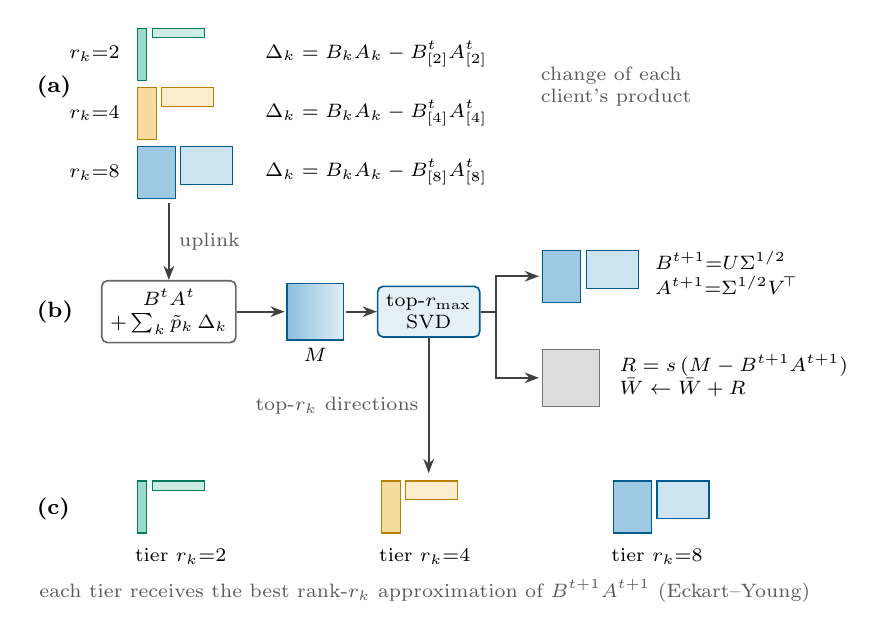
\begin{tikzpicture}[
    font=\scriptsize, >={Stealth[length=1.8mm]},
    flow/.style={->, line width=0.7pt, draw=black!75},
    box/.style={rounded corners=2pt, align=center, inner sep=3pt, line width=0.6pt},
    tag/.style={font=\footnotesize\bfseries, anchor=west},
    pics/lora/.style args={#1/#2}{code={%
        \fill[#2!38, draw=#2!80!black, line width=0.4pt] (0,0) rectangle ++(#1*0.06,-0.66);
        \fill[#2!20, draw=#2!80!black, line width=0.4pt] (#1*0.06+0.07,0) rectangle ++(0.66,-#1*0.06);
    }},
  ]

  % ---------------------------------------------------------------- (a) uploads
  \node[tag] at (-0.55,6.45) {(a)};
  \foreach \rk/\y/\col in {2/7.2/cLoc, 4/6.45/cStat, 8/5.7/cFed} {
    \node[anchor=east] at (0.75,\y-0.33) {$r_k{=}\rk$};
    \pic at (0.85,\y) {lora=\rk/\col};
    \node[anchor=west] at (2.35,\y-0.33) {$\Delta_k=B_kA_k-B^{t}_{[\rk]}A^{t}_{[\rk]}$};
  }
  \node[anchor=west, text=black!65] at (5.85,6.45) {\begin{tabular}{@{}l@{}}change of each\\ client's product\end{tabular}};

  % ---------------------------------------------------------------- (b) server
  \node[tag] at (-0.55,3.6) {(b)};
  \node[box, draw=black!60, fill=white] (sum) at (1.25,3.6) {$B^{t}A^{t}$\\ $+\sum_k\tilde{p}_k\,\Delta_k$};
  \draw[flow] (1.25,4.98) -- node[right, text=black!65]{uplink} (sum.north);
  % dense aggregate M
  \shade[left color=cFed!45, right color=cFed!12, draw=cFed!80!black, line width=0.4pt] (2.75,3.96) rectangle (3.47,3.24);
  \node at (3.11,3.05) {$M$};
  \draw[flow] (sum.east) -- (2.72,3.6);
  \node[box, draw=cFed!80!black, fill=cFed!10] (svd) at (4.55,3.6) {top-$r_{\max}$\\ SVD};
  \draw[flow] (3.5,3.6) -- (svd.west);
  % refactored factors (upper branch) and residual (lower branch)
  \pic at (6.0,4.38) {lora=8/cFed};
  \node[anchor=west] at (7.3,4.05) {\begin{tabular}{@{}l@{}}$B^{t+1}{=}U\Sigma^{1/2}$\\ $A^{t+1}{=}\Sigma^{1/2}V^{\!\top}$\end{tabular}};
  \fill[cFrozen!30, draw=cFrozen!85!black, line width=0.4pt] (6.0,3.12) rectangle (6.72,2.4);
  \node[anchor=west] at (6.85,2.76) {\begin{tabular}{@{}l@{}}$R=s\,(M-B^{t+1}A^{t+1})$\\ $\bar{W}\leftarrow\bar{W}+R$\end{tabular}};
  \draw[flow] (svd.east) -- ++(0.2,0) |- (5.95,4.05);
  \draw[flow] (svd.east) -- ++(0.2,0) |- (5.95,2.76);

  % ---------------------------------------------------------------- (c) download
  \draw[flow] (svd.south) -- node[left, text=black!65]{top-$r_k$ directions} (4.55,1.55);
  \node[tag] at (-0.55,1.1) {(c)};
  \foreach \rk/\x/\col in {2/0.85/cLoc, 4/3.95/cStat, 8/6.9/cFed} {
    \pic at (\x,1.45) {lora=\rk/\col};
    \node[anchor=north] at (\x+0.55,0.72) {tier $r_k{=}\rk$};
  }
  \node[anchor=north, text=black!65] at (4.5,0.32)
       {each tier receives the best rank-$r_k$ approximation of $B^{t+1}A^{t+1}$ (Eckart--Young)};
\end{tikzpicture}
}
  \caption{Exact rank-heterogeneous aggregation for one adapted layer (glyph widths are
  proportional to the rank). (a)~Each client uploads factors of its own rank $r_k$; the server
  forms the change $\Delta_k$ of the client's product relative to what the client received.
  (b)~The weighted mean change is added to the current global product; the result $M$ is
  re-factorized by a truncated SVD at rank $r_{\max}$, and the remainder $R$ is folded into the frozen
  weight, so the effective model equals the aggregate of \cref{prop:exact}. (c)~A device of
  rank $r_k$ receives the leading $r_k$ singular directions.}
  \label{fig:aggregation}
\end{figure}

\subsubsection{Why naive averaging fails}
Averaging the factors separately (FedAvg on $A$ and $B$) does not average the models, because
the product of averages differs from the average of products.

\begin{lemma}[Bias of factor averaging]\label{lem:naive}
Let $\bar{B}=\sum_k\ptil_kB_k$ and $\bar{A}=\sum_k\ptil_kA_k$ with $\sum_k\ptil_k=1$. Then
\begin{equation}\label{eq:naive-bias}
  \bar{B}\bar{A}-\sum_k\ptil_k B_kA_k=-\sum_k\ptil_k\,(B_k-\bar{B})(A_k-\bar{A}).
\end{equation}
\end{lemma}
\begin{IEEEproof}
Expanding the right-hand side gives
$-\sum_k\ptil_kB_kA_k+\bar{B}\bar{A}+\bar{B}\bar{A}-\bar{B}\bar{A}$.
\end{IEEEproof}
The error is a weighted cross-covariance of the client factors. It vanishes only if the clients'
factors do not vary, and it grows precisely when the clients' data differ, i.e., under (H1)--(H2).
FedEx-LoRA~\cite{singhal2025fedex} removes it for equal ranks by adding the residual
$s(\sum_k\ptil_kB_kA_k-\bar{B}\bar{A})$ to the frozen weight. With heterogeneous ranks, however,
two further problems appear: the factors have different shapes, and a low-rank device cannot
represent, and therefore cannot update, the trailing directions of the global adapter.

\subsubsection{Delta-form aggregation}
The server keeps, for every $\ell\in\Lset$, the base $\Wbar^t_\ell$ (initially $\Omega_0$) and
global factors $(B^t_\ell,A^t_\ell)$ at rank $\rmax=\max\mathcal{R}$. We drop the layer index
when no confusion arises. Client $k$ receives the truncated factors
$(\trunc{B^t}{r_k},\trunc{A^t}{r_k})$, trains them, and uploads $(B_k,A_k)$ of rank $r_k$. The server
computes the change of each client's product relative to what that client received,
\begin{equation}\label{eq:delta}
  \Delta_k=B_kA_k-\trunc{B^t}{r_k}\,\trunc{A^t}{r_k},
\end{equation}
adds the weighted mean change to the current global product, re-factorizes the result at rank
$\rmax$ and folds the remainder into the frozen weight:
\begin{align}
  M&=B^tA^t+\sum_{k\in\St}\ptil_k\,\Delta_k, \label{eq:M}\\
  U\Sigma V^{\top}&=\mathrm{SVD}_{\rmax}(M), \nonumber\\
  (B^{t+1},A^{t+1})&=\big(U\Sigma^{1/2},\ \Sigma^{1/2}V^{\top}\big), \label{eq:svd}\\
  \Wbar^{t+1}&=\Wbar^{t}+s\,\big(M-B^{t+1}A^{t+1}\big). \label{eq:residual}
\end{align}
Here $\ptil_k=n_k/\sum_{j\in\St}n_j$ and $\mathrm{SVD}_{\rmax}$ returns the leading $\rmax$ singular
triplets. Directions whose singular value is numerically zero ($\sigma_j<10^{-6}\sigma_1$) would
leave both factors at zero and block their gradients; for these we re-initialize the rows of
$A^{t+1}$ randomly and keep the columns of $B^{t+1}$ at zero, which leaves the product
unchanged. For large matrices ($\min(d^{\mathrm{out}},d^{\mathrm{in}})>4\rmax$) a randomized
SVD~\cite{halko2011finding} with $8$ oversampling vectors and $4$ power iterations is used; as shown
next, this does not affect exactness, because whatever the factors miss is kept in the residual.

\begin{proposition}[Exactness]\label{prop:exact}
Let $W^t=\Wbar^t+sB^tA^t$ be the effective global weight, and let
$W_k^{\mathrm{start}}=\Wbar^t+s\,\trunc{B^t}{r_k}\trunc{A^t}{r_k}$ and
$W_k^{\mathrm{end}}=\Wbar^t+sB_kA_k$ be client $k$'s effective weight before and after local training.
For any ranks $\{r_k\}$ and any factorization returned in \cref{eq:svd},
\begin{equation}\label{eq:exact}
  W^{t+1}=W^t+\sum_{k\in\St}\ptil_k\big(W_k^{\mathrm{end}}-W_k^{\mathrm{start}}\big).
\end{equation}
\end{proposition}
\begin{IEEEproof}
By \cref{eq:residual}, $W^{t+1}=\Wbar^{t+1}+sB^{t+1}A^{t+1}=\Wbar^t+sM$. Substituting \cref{eq:M}
gives $W^{t+1}=\Wbar^t+sB^tA^t+\sum_k\ptil_k\,s\Delta_k=W^t+\sum_k\ptil_k\,s\Delta_k$, and
$s\Delta_k=W_k^{\mathrm{end}}-W_k^{\mathrm{start}}$ by \cref{eq:delta}.
\end{IEEEproof}

\begin{corollary}[Reduction to FedAvg]\label{cor:fedavg}
If all clients use $r_k=\rmax$, then $W_k^{\mathrm{start}}=W^t$ for every $k$, and \cref{eq:exact}
becomes $W^{t+1}=\sum_k\ptil_kW_k^{\mathrm{end}}$: the effective models are averaged exactly as
FedAvg~\cite{mcmahan2017fedavg} would average fully fine-tuned layers, and the rule coincides with
FedEx-LoRA~\cite{singhal2025fedex}.
\end{corollary}

In other words, the server performs FedAvg on the \emph{effective-weight updates} of the clients,
regardless of their ranks and of how the update is factorized. Over rounds, the accumulated
residual lets the global update grow beyond rank $\rmax$, while every device trains only
$r_k(d^{\mathrm{in}}+d^{\mathrm{out}})$ parameters per layer.

\subsubsection{Why the delta form matters}
A natural alternative, used in spirit by product-space methods such as
FlexLoRA~\cite{bai2024flexlora}, averages the zero-padded products,
$M'=\sum_k\ptil_kB_kA_k$. The following property shows that this alternative is biased under rank
heterogeneity, whereas the delta form is not.

\begin{proposition}[Consistency]\label{prop:consistency}
Suppose that, after an aggregation, $B^tA^t=\sum_{j=1}^{\rmax}\sigma_j\mathbf{u}_j\mathbf{v}_j^\top$
is in the balanced SVD form of \cref{eq:svd}, and that no client changes its factors
($B_k=\trunc{B^t}{r_k}$, $A_k=\trunc{A^t}{r_k}$). Then the delta-form rule returns
$W^{t+1}=W^t$, whereas product averaging returns
\begin{equation}\label{eq:shrink}
  M'=\sum_{j=1}^{\rmax}\varrho_j\,\sigma_j\mathbf{u}_j\mathbf{v}_j^\top,\qquad
  \varrho_j=\sum_{k\in\St:\ r_k\ge j}\ptil_k\ \le 1 .
\end{equation}
\end{proposition}
\begin{IEEEproof}
With unchanged factors, $\Delta_k=0$ for all $k$, so $M=B^tA^t$ and $W^{t+1}=W^t$ by
\cref{prop:exact}. For product averaging, the balanced form gives
$\trunc{B^t}{r}\trunc{A^t}{r}=\sum_{j\le r}\sigma_j\mathbf{u}_j\mathbf{v}_j^\top$; summing over clients
with weights $\ptil_k$ and exchanging the sums yields \cref{eq:shrink}.
\end{IEEEproof}
Under product averaging, the $j$-th direction of the global adapter is therefore multiplied by
$\varrho_j$ in every round, independently of the data. With tiers drawn uniformly from $\{2,4,8\}$,
$\E[\varrho_j]=1,\ \tfrac{2}{3},\ \tfrac{1}{3}$ for $j\in\{1,2\}$, $\{3,4\}$ and $\{5,\dots,8\}$: what the
high-tier devices learn is diluted geometrically by the low-tier devices that never hold those
directions. In the delta form, a client that does not hold a direction contributes a zero
\emph{change} to it rather than a zero \emph{value}. Finally, because $(B^t,A^t)$ is in balanced SVD
form, the truncation sent to a rank-$r_k$ device is the best rank-$r_k$ approximation of the global
adapter in the Frobenius and spectral norms (Eckart--Young--Mirsky~\cite{eckart1936approximation}):
weak devices receive the most informative part of the global update.

% ---------------------------------------------------------------------
\subsection{Aggregation of the Head, Prototypes and Statistics}\label{sec:method:stats}

The projection head is averaged as $\theta^{t+1}=\sum_{k\in\St}\ptil_k\theta_k$. Prototypes are
aggregated with the class counts as weights,
\begin{equation}\label{eq:global-proto}
  \mathbf{P}_c=\frac{\sum_{k\in\St}n_{k,c}\,\mathbf{p}_{k,c}}{\sum_{k\in\St}n_{k,c}},
\end{equation}
so a client contributes to a class only if it observes that class; a class that no participant
observes in a round keeps its previous prototype. In addition, every client uploads two
statistics once, before training: its class counts $\{n_{k,c}\}_c$ and its activity-transition
counts $N_k\in\mathbb{N}^{C\times C}$, computed from its chronologically ordered training labels.
The server forms the global prior $\pi_c\propto\sum_kn_{k,c}$ and the transition matrix of the
temporal decoder (\cref{sec:method:inference}). Together these statistics cost
$C^2+C=42$ integers per client.

% ---------------------------------------------------------------------
\subsection{Learning under Label Skew}\label{sec:method:skew}

\subsubsection{Why rare classes vanish with a shared classifier}
With a shared classifier $f$ and plain cross-entropy, the gradient with respect to the logit of
class $c$ is $q_c-\mathbf{1}[y=c]$, where $q=\mathrm{softmax}(f(\mathbf{x}))$. On a client that
never observes $c$, every sample therefore lowers the logit of $c$. When a class is absent on
most clients, averaging their updates erases it from the global model. In our earlier experiments
on the free-living Capture-24 dataset~\cite{chan2024capture24}, where three quarters of the users
never cycle, $35$ of the $168$ per-class F1 scores of the federated models were zero without the
remedies described below. HARBox is far less skewed (\cref{sec:data:hetero}), but some users still
lack one or two activities.

\subsubsection{\method}
The proposed design avoids this structurally: the classifier is personal (\ding{176}), so no
client's decision rule is pulled towards other clients' priors. The only shared class-specific
quantities are the prototypes, and \cref{eq:global-proto} averages each prototype only over the
clients that have the class.

\subsubsection{Shared-classifier methods}
So that the comparison with methods that share the classifier (V0--V4 in \cref{tab:methods}) is
not dominated by the class-imbalance problem, those methods are equipped with three standard
remedies. First, every client trains with a logit-adjusted (balanced-softmax)
loss~\cite{menon2021logit,ren2020balanced,zhang2022fedlc} that uses its \emph{own} prior,
\begin{equation}\label{eq:la}
  \ell(\mathbf{x},y)=\CE\big(f(\mathbf{x})+\tau\log\boldsymbol{\pi}_k,\ y\big),\qquad\tau=1,
\end{equation}
where $\boldsymbol{\pi}_k$ is floored at $10^{-4}$. The gradient for an absent class becomes
$q'_c\propto\pi_{k,c}^{\tau}e^{f_c}\approx 10^{-4}e^{f_c}$, so absent classes are no longer pushed
down, and $f$ learns class-balanced scores. Second, the rows of the shared classifier are
aggregated class-wise~\cite{li2021fedrs,shang2022creff},
\begin{equation}\label{eq:classwise}
  [W]_c^{t+1}=\frac{\sum_{k\in\St}n_{k,c}[W_k]_c}{\sum_{k\in\St}n_{k,c}}\quad\text{(the same for $b_c$)},
\end{equation}
and a row that no participant observes keeps its value. Third, decisions are calibrated with
the global prior (\cref{eq:calibrated}). Full-model methods (FedAvg and V0) also use a larger
learning rate for the heads than for the body (discriminative learning rates), without which
the rows of rare classes barely move within the training budget.

% ---------------------------------------------------------------------
\subsection{Inference}\label{sec:method:inference}

\subsubsection{Enrolled users}
\method{} predicts $\hat{y}=\arg\max_c[h_k(\mathbf{e})]_c$ with the user's rank, local parts and
personal head. A shared classifier trained with \cref{eq:la} outputs class-balanced scores, which
we convert into decisions with a tunable prior strength,
\begin{equation}\label{eq:calibrated}
  \hat{y}=\arg\max_c\ f_c(\mathbf{x})+\tau_{\mathrm{inf}}\log\pi_c .
\end{equation}
$\tau_{\mathrm{inf}}=0$ gives balanced decisions and $\tau_{\mathrm{inf}}=1$ the accuracy-optimal
decisions under $\boldsymbol{\pi}$; macro-F1 is best in between. We select
$\tau_{\mathrm{inf}}=0.5$ from $\{0,0.25,0.5,0.75,1\}$ on the validation users and keep it fixed for all
methods and encoders.

\subsubsection{Federated temporal decoding (continuous streams)}
In free-living data, activities last minutes to hours, whereas the classifier sees a single
window. Following the Capture-24 benchmark~\cite{chan2024capture24,walmsley2022reallocation}, \method{}
can therefore decode each
user's chronological sequence with a hidden Markov model (HMM) whose hidden states are the
activities. The transition matrix is estimated from the aggregated counts with add-one smoothing,
$\Gamma_{ij}=(1+\sum_kN_{k,ij})/\sum_{j'}(1+\sum_kN_{k,ij'})$, so it is learned federatedly from
$C^2$ integers per client without sharing any label sequence. The emission score of window
$\mathbf{x}$ for state $c$ is the class-balanced score,
\begin{equation}\label{eq:emission}
  \log p(\mathbf{x}\mid c)\simeq\log\mathrm{softmax}\big(f(\mathbf{x})-(1-\tau)\log\tilde{\boldsymbol{\pi}}\big)_c,
\end{equation}
with $\tau=1$ and $\tilde{\boldsymbol{\pi}}=\boldsymbol{\pi}$ for a logit-adjusted shared classifier. For a
personal classifier ($\tau=0$) we divide by the client's prior shrunk halfway towards the global
one, $\tilde{\boldsymbol{\pi}}=\tfrac12\boldsymbol{\pi}_k+\tfrac12\boldsymbol{\pi}$; dividing by
$\boldsymbol{\pi}_k$ alone would boost classes that the client has never observed by up to
$-\log10^{-4}\approx9$\,nats. The Viterbi algorithm~\cite{viterbi1967error} returns the most likely
activity sequence in $\mathcal{O}(|\Dk^{\mathrm{te}}|\,C^2)$ time. Sequences are split wherever two
consecutive windows are more than three nominal spacings apart, so the decoder never smooths across
recording gaps. Decoding runs on the device; it uses only the shared $\Gamma$ and $\boldsymbol{\pi}$.

\subsubsection{New users}
A user $u$ who never participated downloads the global state (rank $\rmax$) and the prototypes.
Its local parts must be initialized. The pretrained normalization and adapter do not match the
representation that the federated LoRA and head were trained with, because every client trained
its own. Therefore, once at the end of training, every client uploads its local normalization
parameters and input adapter (not its personal classifier), and the server keeps their
$n_k$-weighted average $\bar{\psi},\bar{a}$ as the initialization for new users. On LIMU-BERT this
costs a one-time upload of $2$\,kB per client and raises the new-user scores at every label budget
(\cref{sec:results:newusers}).
\emph{Zero-shot}: encoders with BatchNorm additionally re-estimate their normalization statistics on
the user's \emph{unlabelled} windows (AdaBN~\cite{li2018adabn}); the user is then served by the
nearest-prototype rule
\begin{equation}\label{eq:zeroshot}
  \hat{y}=\arg\max_{c\in\mathcal{C}_P}\ \cos\big(\mathbf{e},\mathbf{P}_c\big).
\end{equation}
\emph{Transductive zero-shot} (optional). The global prototypes describe the federation, not the
new user. Before serving, the device can move them towards its own unlabelled windows
$\{\mathbf{z}_i\}$ (unit-norm embeddings of the same windows AdaBN uses) with $T$ soft $k$-means
steps anchored at the global prototypes $\hat{\mathbf{P}}^{(0)}_c=\mathbf{P}_c/\norm{\mathbf{P}_c}$:
\begin{equation}\label{eq:refine}
\begin{aligned}
  w_{ic}&=\operatorname{softmax}_{c\in\mathcal{C}_P}\big(\mathbf{z}_i^\top\hat{\mathbf{P}}^{(t)}_c/\vartheta\big),\\
  \hat{\mathbf{P}}^{(t+1)}_c&=\mathbf{m}_c/\norm{\mathbf{m}_c},\quad
  \mathbf{m}_c=\textstyle\sum_i w_{ic}\,\mathbf{z}_i+\kappa\,\hat{\mathbf{P}}^{(0)}_c,
\end{aligned}
\end{equation}
and then applies \cref{eq:zeroshot} with $\hat{\mathbf{P}}^{(T)}$. The anchor weight $\kappa$, in windows,
keeps a class the user rarely performs close to its global prototype; without it ($\kappa=0$) the
clusters drift away from their classes. This is the prototype counterpart of test-time classifier
adjustment~\cite{iwasawa2021t3a}: it uses no labels, no communication and no gradient step. We use
$T=10$, $\vartheta=0.1$ and $\kappa=10$, selected on the validation users. Applied to the
normalized class weights of a shared classifier, the same update lowers the validation zero-shot
score, so the baselines keep their own classifier.
\emph{Few-shot}: with $m$ minutes of labels per activity, a new personal head is initialized at the
zero-shot solution, $[W_u]_c=\mathbf{P}_c/\norm{\mathbf{P}_c}$ and $b_{u,c}=0$ (with the refined
prototypes when the transductive rule is used), since
$\arg\max_c\cos(\mathbf{e},\mathbf{P}_c)=\arg\max_c\mathbf{P}_c^\top\mathbf{e}/\norm{\mathbf{P}_c}$. The head, the
norms and the input adapter $\{h_u,\psi_u,a_u\}$ are then fine-tuned on the shots. BatchNorm
statistics stay fixed at their AdaBN estimates during this fit: the scale and shift of $\psi_u$
adapt to the labels, but the statistics come from all of the user's unlabelled windows, not from a
batch of a few shots. Because the
shots are roughly class-balanced, unlike a real day, this fit uses \cref{eq:la} with the prior of
the shots, and decisions use \cref{eq:calibrated}.

% ---------------------------------------------------------------------
\subsection{Training-Time Augmentation}\label{sec:method:augment}

The same device can be held at many angles, and different devices use different axis
conventions. During local training, each window is therefore transformed, with probability $p$,
by one random rotation $R\in SO(3)$ (uniform axis, angle up to $\theta_{\max}$) and a random gain $g$:
$\mathbf{x}_{s}\leftarrow g\,R\,\mathbf{x}_{s}$ for every sensor triplet $s$ (accelerometer, gyroscope,
magnetometer). The same $R$ is applied to all triplets, as for a rotated phone. The
transformation acts on the stored windows before $\Pi_E$, so it is identical for every encoder and
method, and it costs one batched $C\times C$ matrix product per mini-batch.

% ---------------------------------------------------------------------
\subsection{Training Procedure}\label{sec:method:algorithm}

\Cref{alg:fedpeft} summarizes training. Each device is assigned a rank tier once, and each round
consists of download, local training of the trainable roles, prototype computation, upload of
the federated roles and statistics, and server aggregation. Because only a fraction $\rho$ of the
clients participates in a round, the personal parts of a client may lag behind the latest global
representation. After the last round, every client therefore performs a short personalization
pass ($8$ steps) that updates only $\phi_k$ against the final global model, without any
communication.

\begin{algorithm}[!t]
\caption{\method{} training}
\label{alg:fedpeft}
\footnotesize
\SetKwInOut{Input}{Input}\SetKwInOut{Output}{Output}
\SetKwFor{ForPar}{for}{in parallel do}{end}
\SetCommentSty{textit}
\Input{clients $k=1..K$ with $\Dk^{\mathrm{tr}}$; tiers $\mathcal{R}$; rounds $T$; rate $\rho$; local steps $S$; weight $\lambda$; pretrained $\Omega_0$}
\Output{global state $(\{\Wbar_\ell,B_\ell,A_\ell\}_\ell,\theta,\{\mathbf{P}_c\},\boldsymbol{\pi},\Gamma)$; local parts $\{\phi_k\}$}
\textbf{Server:} $\Wbar_\ell\gets\Omega_{0,\ell}$, $B_\ell\gets0$, $A_\ell\gets\mathrm{Kaiming}(\rmax)$, $\theta\gets$ init, $\mathcal{C}_P\gets\emptyset$\;
\For{each client $k$}{
  $r_k\sim\mathrm{Uniform}(\mathcal{R})$;\ \ $\phi_k\gets(\text{identity }a_k,\ \text{pretrained }\psi_k,\ \text{random }h_k)$\;
  send $\{n_{k,c}\}_c$ and $N_k$ to the server \tcp*{once}
}
\textbf{Server:} build the prior $\boldsymbol{\pi}$ and the HMM transitions $\Gamma$\;
\For{$t=0,\dots,T-1$}{
  $\St\gets$ random subset of $\lceil\rho K\rfloor$ clients\;
  \ForPar{$k\in\St$}{
    receive $\{\Wbar_\ell,B_{\ell,[r_k]},A_{\ell,[r_k]}\}_{\ell}$, $\theta$, $\{\mathbf{P}_c\}_{c\in\mathcal{C}_P}$\;
    $S$ AdamW steps on $F_k$ (\cref{eq:local-obj}) w.r.t.\ $\{A_\ell,B_\ell\},\theta,\phi_k$\;
    compute $\mathbf{p}_{k,c}$ by \cref{eq:local-proto}; keep $\phi_k$ on the device\;
    upload $\{A_{k,\ell},B_{k,\ell}\}_\ell$, $\theta_k$, $\{\mathbf{p}_{k,c},n_{k,c}\}_c$, $n_k$\;
  }
  \textbf{Server:} for every $\ell\in\Lset$ apply \cref{eq:delta,eq:M,eq:svd,eq:residual}\;
  \textbf{Server:} $\theta\gets\sum_k\ptil_k\theta_k$; prototypes by \cref{eq:global-proto}\;
}
\For(\tcp*[f]{final personalization, no communication}){each client $k$}{
  $8$ steps on $F_k$ w.r.t.\ $\phi_k$ only, at the final global state\;
}
\end{algorithm}

% ---------------------------------------------------------------------
\subsection{Communication, Memory and Computation}\label{sec:method:cost}

\subsubsection{Uplink}
Per round, client $k$ uploads
\begin{equation}\label{eq:uplink}
  U_k=\underbrace{r_k\textstyle\sum_{\ell\in\Lset}\big(d^{\mathrm{in}}_\ell+d^{\mathrm{out}}_\ell\big)}_{\text{LoRA}}
  +\underbrace{|\theta|}_{\text{head}}+\underbrace{C(D+1)}_{\text{prototypes, counts}}
\end{equation}
values, which is linear in the rank and independent of the size of the frozen encoder. Full
fine-tuning uploads $|\Omega_0|+|\theta|+|h|$ values. \Cref{tab:budget} lists the resulting budgets
for the four encoders on HARBox together with the measured uplink: \method{} sends
$\ResUplinkRatioMin\times$ (LIMU-BERT, the smallest encoder) to $\ResUplinkRatioMax\times$ fewer bytes per
update than full fine-tuning, and the factor grows with the size of the encoder.

\subsubsection{Downlink}
In addition to the truncated factors, the head and the prototypes, exact aggregation changes the
frozen weights $\Wbar_\ell$, which a client must receive before it trains again. In our accounting we
conservatively charge the full dense $\Wbar_\ell$ of every adapted layer at each download. This term
can be reduced substantially: if the truncated SVD in \cref{eq:svd} is exact, the per-round residual
in \cref{eq:residual} has rank at most $\sum_{k\in\St}r_k$, because
$\mathrm{rank}(M)\le\rmax+\sum_{k\in\St}r_k$, and it can therefore be transmitted in factored form.
We report the conservative figure and return to this point in the discussion.

\subsubsection{Client memory and computation}
Only LoRA factors, the heads and $\phi_k$ require gradients and optimizer states, i.e., three
additional floating-point values per trainable parameter for AdamW~\cite{loshchilov2019adamw}.
Activation memory still scales with the encoder, so the memory saving is largest when the
optimizer state dominates (large convolutional encoders) and modest for small Transformers.
Prototype computation needs one extra forward pass over at most $512$ windows per round.

\subsubsection{Server computation}
Forming $M_\ell$ costs $\mathcal{O}\big(d^{\mathrm{out}}_\ell d^{\mathrm{in}}_\ell\sum_{k\in\St}r_k\big)$, and the
randomized SVD costs $\mathcal{O}\big(d^{\mathrm{out}}_\ell d^{\mathrm{in}}_\ell(\rmax+8)\big)$ per layer and
round. The server streams the uploads into running sums, so its memory does not grow with the
number of participating clients.

\begin{table*}[!t]
\centering
\caption{Parameter budget per encoder on HARBox and measured communication per client update
(fp32 serialization, no compression). $|\Omega_0|$: frozen encoder weights; LoRA: trainable
adapter parameters at rank $r=2/4/8$; $|\theta|$: shared head; $|\phi_k|$: local parameters
(norm affine, adapter, classifier).}
\label{tab:budget}
\footnotesize
\setlength{\tabcolsep}{4.2pt}
\renewcommand{\arraystretch}{1.12}
\begin{tabular}{@{}l l r r r r c c r@{}}
\toprule
Encoder & LoRA targets & $|\Omega_0|$ & LoRA ($r{=}2/4/8$) & $|\theta|$ & $|\phi_k|$
  & \makecell{Uplink \method\\ $r{=}2/4/8$ (MB)} & \makecell{Uplink full FT\\ (MB)} & \makecell{Ratio$^{\dagger}$} \\
\midrule
\inputrows{generated/res_tab_budget.tex}
\bottomrule
\end{tabular}

\vspace{2pt}
\begin{minipage}{\textwidth}\footnotesize
$^{\dagger}$Mean uplink of full fine-tuning divided by the mean uplink of \method{} over all client updates
(tiers drawn uniformly). $^{\ddagger}$Our re-implementation of the HALO encoder, pretrained
self-supervised on the pool users (\cref{sec:data:encoders}).
\end{minipage}
\end{table*}

% ---------------------------------------------------------------------
\subsection{Privacy Considerations}\label{sec:method:privacy}

Raw windows, labels, label sequences, local normalization statistics, input adapters and personal
classifiers never leave the device. The uploads are the LoRA factors and the projection head (as
in any PEFT-based federated method), $C$ class-mean embeddings in a $64$-dimensional space and
their counts, and, once, $C+C^2$ label statistics. Prototypes and counts reveal which activities
a user performed, so they are as sensitive as a coarse activity diary; they can be protected by
adding calibrated Gaussian noise to $\mathbf{p}_{k,c}$ and $n_{k,c}$ or by aggregating them with secure
aggregation~\cite{bonawitz2017practical}, because \cref{eq:global-proto} is a ratio of two sums.
The products $B_kA_k$ in \cref{eq:M} are also sums over clients, but secure aggregation of their dense
form would forgo the uplink savings. A formal privacy analysis is beyond the scope of this work.

% =====================================================================
%  Section IV - Dataset and experimental protocol (HARBox)
%  All numbers come from paper/generated/harbox_*.tex
%  (scripts/tools/paper_harbox_stats.py) or from configs/datasets/harbox.yaml
%  and configs/profiles/harbox*.yaml.
%  The previous Capture-24 version of this section is kept in dataset_capture24.tex.
% =====================================================================
\section{Dataset and Experimental Protocol}\label{sec:data}

% ---------------------------------------------------------------------
\subsection{The HARBox Dataset}\label{sec:data:harbox}

We evaluate on HARBox~\cite{ouyang2021clusterfl}, the largest of the federated HAR datasets
released with ClusterFL. Unlike laboratory collections, it was \emph{crowd-sourced}: volunteers
installed an Android application on their own smartphones and recorded five activities of daily
life, labelling each recording themselves by pressing ``start'' and ``end'' in the
application (\cref{tab:classes}). After invalid and repeated submissions were removed, the data
of $121$ users aged $17$--$55$ years remained, recorded with $77$ different smartphone models. Each
recording contains the $9$-axis inertial signals of the phone (tri-axial accelerometer in
m\,s$^{-2}$, gyroscope in rad\,s$^{-1}$ and magnetometer in $\mu$T), resampled by the authors to
$50$\,Hz and cut into $2$\,s windows with a $1$\,s hop, so consecutive windows of a recording
overlap by $50\,\%$. One user has no windows. The remaining $\HBUsers{}$ users contribute
$\HBWindows{}$ windows (about $\HBHours{}$\,h of distinct signal). Users and phones are the natural
unit of federation, so every user is one client and no synthetic partition is needed. The
heterogeneity that federated HAR must handle (different devices, grips, body sizes and
movement styles) is present by construction.

\begin{table}[!t]
\centering
\caption{HARBox activities after windowing ($2$\,s windows, $50$\,Hz, $9$ axes), over all
\HBUsers{} users. Users: users with at least one window of the activity.}
\label{tab:classes}
\footnotesize
\setlength{\tabcolsep}{4pt}
\renewcommand{\arraystretch}{1.1}
\begin{tabularx}{\columnwidth}{@{}l Y r r r@{}}
\toprule
Activity & Description & Windows & \% & Users \\
\midrule
\inputrows{generated/harbox_tab_classes.tex}
\bottomrule
\end{tabularx}
\end{table}

\begin{figure*}[!t]
  \centering
  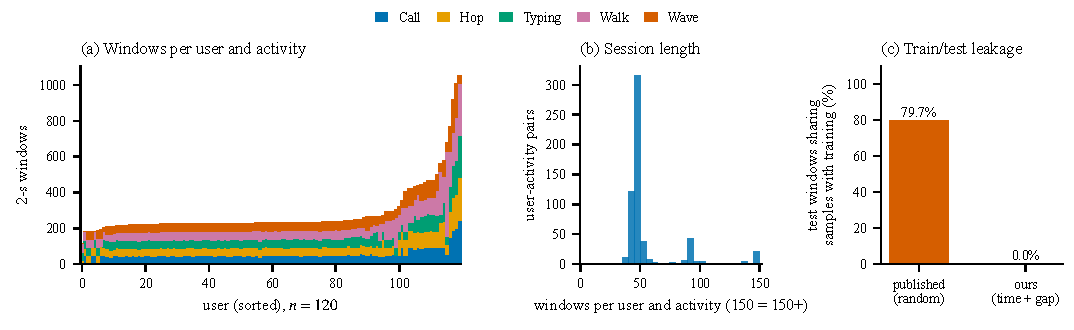
\includegraphics[width=\textwidth]{figures/harbox_stats.pdf}
  \caption{HARBox at a glance. (a)~Windows per user and activity: users differ in how long they
  recorded, not in which activities. (b)~Length of the recording of one activity by one user,
  typically below one minute. (c)~Share of test windows that overlap a training window by half of
  their samples. The random split of the published protocol leaks the large majority; our
  per-activity chronological split with a one-window gap leaks none.}
  \label{fig:harbox}
\end{figure*}

% ---------------------------------------------------------------------
\subsection{Preprocessing}\label{sec:data:preprocessing}

We use the windows exactly as released: each window is a $9\times100$ array in physical units,
ordered by its start time, and assigned the activity of the file it comes from. We also
reconstruct the recording session of each window from the timestamps: a new session starts
wherever two consecutive windows of an activity start more than $1.5$\,s apart. The median user
contributes $\HBWinUserClassMedian{}$ windows per activity, i.e., less than one minute of
recording, in a median of five sessions. No resampling or filtering is applied at storage time.
The encoder-specific preprocessing $\Pi_E$ (\cref{sec:method:client}) converts units, resamples to
the encoder's rate and fits the window length (\cref{tab:encoders}). Only the training windows
are augmented (\cref{sec:data:impl}).

% ---------------------------------------------------------------------
\subsection{Evaluation Protocols}\label{sec:data:splits}

Two protocols are used (\cref{tab:partition}).

\emph{Protocol A (published).} To compare with published results, we reproduce the protocol of
FedCHAR~\cite{li2023fedchar}: every user is a client, draws a random number of $50$ to $500$ of its
windows, and splits them at random into $72\,\%$ training, $8\,\%$ validation and $20\,\%$ test
windows. Training runs for $100$ rounds with half of the users per round, and the metric is the
mean test accuracy over users. Because consecutive windows overlap by $50\,\%$, however, a random
split places at least one neighbour of most test windows in the training set. We measured that
$\HBLeakA\,\%$ of the test windows share half of their samples with a training window
(\cref{fig:harbox}c). Protocol~A therefore rewards memorizing a user's recordings rather than
recognizing the activity, and we use it only for the comparison with published numbers.

\emph{Protocol B (ours, leakage-free).} The $\HBUsers$ users are randomly assigned, with a fixed
seed, to $\HBClientsB$ FL clients ($70\,\%$), $\HBHeldoutB$ held-out users ($20\,\%$) and $\HBPoolB$
pool users ($10\,\%$). Every activity of a client is split \emph{in time}: the first $80\,\%$ of its
windows are used for training and the last $20\,\%$ for testing. The window between the two
parts is discarded, because it overlaps both. A plain chronological split of the whole recording
would put entire activities into the test part, since HARBox records each activity in its own
session. No test window overlaps a training window, and every activity of a client appears on
both sides. The held-out users never take part in training. For each of their activities, the
first half is the pool from which few-shot labels may be drawn and the second half is the test
set (again with a one-window gap). The pool users provide unlabelled data for the
self-supervised pretraining of HALO and serve as validation users for model selection. No test
data are used for any choice. All main results of this paper use Protocol~B. LIMU-BERT and the MLP
baselines are repeated on two further user splits (seeds $1$ and $2$, \cref{tab:seeds}).

\begin{table}[!t]
\centering
\caption{The two evaluation protocols on HARBox (seed $0$). $^{\dagger}$Pool users' windows (validation).}
\label{tab:partition}
\footnotesize
\setlength{\tabcolsep}{3pt}
\renewcommand{\arraystretch}{1.12}
\begin{tabularx}{\columnwidth}{@{}>{\raggedright\arraybackslash}p{2.3cm} Y Y@{}}
\toprule
 & Protocol B (ours) & Protocol A (published) \\
\midrule
\inputrows{generated/harbox_tab_partition.tex}
\bottomrule
\end{tabularx}
\end{table}

% ---------------------------------------------------------------------
\subsection{Statistical Heterogeneity}\label{sec:data:hetero}

HARBox differs from free-living datasets in where its heterogeneity lies (\cref{tab:hetero}).
Label skew is mild: $112$ of the $\HBUsers$ users recorded all five activities, and a user's
label distribution diverges from the global one by only $\HBJSD$ bits on average. Quantity skew is
substantial ($\HBWinUserMin$ to $\HBWinUserMax$ windows per user). The dominant heterogeneity is in
the signals themselves. Seventy-seven phone models with different sensor ranges, noise levels and
axis conventions are held, pocketed and waved by $\HBUsers$ different people, each recording every
activity only once and for less than a minute. The class-conditional distributions
$p_k(\mathbf{x}\mid y)$ therefore differ strongly between users (heterogeneity~(H2) in
\cref{sec:method:problem}), and they can be learned only from very little data per user. This is
the regime that the local normalization, the local input adapter and the personal classifier of
\method{} are designed for. The label-skew remedies of \cref{sec:method:skew} matter less here.

\begin{table}[!t]
\centering
\caption{Statistical heterogeneity of the \HBUsers{} HARBox users. JSD: Jensen--Shannon divergence in bits.}
\label{tab:hetero}
\footnotesize
\renewcommand{\arraystretch}{1.1}
\begin{tabularx}{\columnwidth}{@{}Y r@{}}
\toprule
Statistic & Value \\
\midrule
\inputrows{generated/harbox_tab_hetero.tex}
\bottomrule
\end{tabularx}
\end{table}

% ---------------------------------------------------------------------
\subsection{Pretrained Encoders}\label{sec:data:encoders}

To test whether the conclusions depend on the backbone, we instantiate \method{} with four IMU
encoders that differ in architecture (Transformer, residual CNN, spatio-temporal graph network,
patch-channel Transformer), size ($51$\,k to $10.4$\,M frozen parameters), pretraining corpus and
objective, and input format (\cref{tab:encoders}). We add the multilayer perceptron of the published
HARBox results~\cite{ouyang2021clusterfl,li2023fedchar} as a from-scratch reference. Three encoders use their official
checkpoints, loaded into re-implementations with identical parameter names (loading fails if
less than $90\,\%$ of the tensors match). LIMU-BERT was pretrained on smartphone data with
accelerometer and gyroscope~\cite{stisen2015smart}, the closest match to HARBox. Its 120 position
embeddings cover $6$\,s at $20$\,Hz, of which a $2$\,s window uses the first $40$. ssl-wearables expects
$10$\,s at $30$\,Hz, so the resampled $2$\,s window is repeated five times. UniMTS receives the
accelerometer on the right-wrist joint of its 22-joint skeleton, the joint closest to a
hand-held phone. HALO~\cite{ding2026halo} has not released weights. We re-implemented its encoder at a
reduced width ($d=192$) and pretrained it with its stage-1 objectives (masked reconstruction of
$50\,\%$ of the patches~\cite{he2022masked} and a patch-level InfoNCE loss~\cite{oord2018representation})
on the unlabelled windows of the pool users, with all nine axes and $0.4$\,s patches. Because HALO
tokenizes every channel separately, it is the only pretrained encoder that uses the magnetometer
from the start. The input adapters of the others may learn to mix it in.

\begin{table*}[!t]
\centering
\caption{Encoders and their HARBox input. Input: channels after the input adapter, sampling
rate, samples (duration) and units, produced from the stored $9\times100$ window by $\Pi_E$.}
\label{tab:encoders}
\footnotesize
\setlength{\tabcolsep}{4pt}
\renewcommand{\arraystretch}{1.15}
\begin{tabularx}{\textwidth}{@{}l Y Y l r r@{}}
\toprule
Encoder & Architecture & Pretraining data and objective & HARBox input & $d_z$ & $|\Omega_0|$ \\
\midrule
LIMU-BERT~\cite{xu2021limubert} &
  Transformer, 4 weight-shared layers (ALBERT-style), $d=72$, 4 heads, mean pooling &
  HHAR smartphones and smartwatches~\cite{stisen2015smart}; masked-span reconstruction (official checkpoint) &
  6 (acc+gyro), 20\,Hz, 40 (2\,s), $g$ & 72 & 51\,k \\
ssl-wearables~\cite{yuan2024selfsupervised} &
  1-D ResNet-V2 (harnet10), 5 stages, 64--1024 channels, anti-aliased down-sampling &
  UK Biobank, 700\,k person-days of wrist accelerometry; multi-task self-supervision &
  3 (acc), 30\,Hz, 60 tiled to 300, $g$ & 1024 & 10.4\,M \\
UniMTS~\cite{zhang2024unimts} &
  ST-GCN~\cite{yan2018spatial}, 10 blocks over a 22-joint skeleton graph, 64--512 channels &
  IMU synthesized from motion capture (HumanML3D~\cite{guo2022generating}); contrastive text alignment &
  3 (acc) on wrist joint, 20\,Hz, 40, m\,s$^{-2}$ & 512 & 5.2\,M \\
HALO~\cite{ding2026halo} (re-impl.) &
  0.4-s patch $\times$ channel tokens, 8 alternating temporal/cross-channel attention layers, $d=192$, query pooling &
  HARBox pool users (unlabelled, disjoint from all evaluation users); masked reconstruction + patch contrastive &
  9 (acc+gyro+mag), 50\,Hz, 100, $g$ & 256 & 4.6\,M \\
MLP~\cite{li2023fedchar} &
  flattened window, one hidden layer of 300 units (the published HARBox model) &
  none (trained from scratch) &
  9, 50\,Hz, 100 (900 features) & 300 & -- \\
\bottomrule
\end{tabularx}
\end{table*}

% ---------------------------------------------------------------------
\subsection{Compared Methods}\label{sec:data:methods}

\Cref{tab:methods} lists the federated methods, each defined by the roles of \cref{tab:roles}.
FedAvg trains the whole model from a random initialization. V0 and V1 are the upper-cost and
lower-cost ways of using a pretrained encoder (full fine-tuning; a frozen encoder with trainable
heads). V2 and V3 isolate the aggregation rule for homogeneous LoRA: factor averaging versus
exact aggregation~\cite{singhal2025fedex}. V4 adds rank heterogeneity with the delta-form
aggregation of \cref{sec:method:agg}, and it is the ablation of \method{} (V5) without local parts and
prototypes. The MLP is trained with the baselines of the published HARBox results: FedAvg, purely
local training, and Ditto~\cite{li2021ditto}, the personalized method on which FedCHAR
builds. Because Ditto is the strongest of these, we also run it from the pretrained LIMU-BERT
(Ditto, pretrained), which gives the personalized full-model baseline at the communication cost of
V0. Every method uses the same augmentation, decoders and evaluation. Two centralized
references are trained on the pooled training parts of the clients: \emph{from scratch}, which
defines the target accuracy, and \emph{pretrained fine-tuning}, an upper reference without privacy
constraints.

\begin{table*}[!t]
\centering
\caption{Federated methods. $\Omega$: encoder weights; $g$, $h$: shared and classifier heads;
$\psi$: normalization; $a$: input adapter; P: prototypes.}
\label{tab:methods}
\footnotesize
\setlength{\tabcolsep}{4.5pt}
\renewcommand{\arraystretch}{1.12}
\begin{tabular}{@{}l l l l l l l@{}}
\toprule
Method & Init. & Trained & Uploaded & Kept local & LoRA rank & Aggregation \\
\midrule
Local & random & $\Omega,\psi,a,g,h$ & -- & everything & -- & none \\
FedAvg~\cite{mcmahan2017fedavg} & random & $\Omega,\psi,a,g,h$ & $\Omega,\psi,a,g,h$ & -- & -- & FedAvg \\
Ditto~\cite{li2021ditto} & random & global + personal copy & $\Omega,\psi,a,g,h$ & personal copy & -- & FedAvg + proximal personal model \\
V0 Full fine-tuning & pretrained & $\Omega,\psi,a,g,h$ & $\Omega,\psi,a,g,h$ & -- & -- & FedAvg \\
Ditto, pretrained & pretrained & global + personal copy & $\Omega,\psi,a,g,h$ & personal copy & -- & FedAvg + proximal personal model \\
V1 Head only & pretrained & $g,h$ & $g,h$ & -- & -- & FedAvg \\
V2 LoRA, factor averaging & pretrained & LoRA, $g,h$ & LoRA, $g,h$ & -- & 8 & avg.\ $A$, avg.\ $B$ \\
V3 LoRA, exact & pretrained & LoRA, $g,h$ & LoRA, $g,h$ & -- & 8 & FedEx-LoRA~\cite{singhal2025fedex} \\
V4 Heterogeneous ranks & pretrained & LoRA, $g,h$ & LoRA, $g,h$ & -- & 2/4/8 & delta form + SVD (\cref{sec:method:agg}) \\
\textbf{V5 \method} & pretrained & LoRA, $g,h,\psi,a$ & LoRA, $g$, P & $h,\psi,a$ & 2/4/8 & delta form + SVD, prototypes \\
\bottomrule
\end{tabular}
\end{table*}

% ---------------------------------------------------------------------
\subsection{Evaluation Metrics}\label{sec:data:metrics}

\emph{Recognition.} Following the published HARBox results, the primary metric is the \emph{mean
per-user accuracy}, i.e., the test accuracy of every client averaged over clients. We also report
the macro-F1 over the five activities, computed on the pooled test windows of all clients.

\emph{Fairness.} We report the mean accuracy of the $\lceil0.1K\rceil$ worst-served clients
(\emph{worst-10\,\%}) and the standard deviation of the per-client macro-F1 over the activities
present in each client's test part.

\emph{Communication.} Every message is an explicit set of tensors whose size is measured as the
serialized size of uncompressed arrays (four bytes per real value, eight per integer), as in
Flower's NumPy serialization~\cite{beutel2020flower}. It includes every tensor that is sent:
factors, heads, residual weights, prototypes and counts. We report the uplink per client update
(MB), the rounds to target (the first evaluated round whose macro-F1 reaches $90\,\%$ of the
centralized from-scratch macro-F1 of the same encoder) and the cumulative uplink up to that round.
No compression or quantization is applied.

\emph{Client cost.} The client memory is the size of all model tensors plus the peak additional
device memory allocated during a local update, measured with the CUDA allocator. The client time
is the wall-clock time of one local update.

\emph{New users (Protocol B).} On the \HBHeldoutB{} held-out users we report the mean per-user
macro-F1 on their test parts: zero-shot (no labels) and few-shot with $1$, $5$ and $10$ labelled
windows ($2$, $10$ and $20$\,s) per activity, drawn at random from their adaptation parts.

\emph{Personalized evaluation.} Methods with a shared classifier are also scored after the common
``FedAvg + local fine-tuning'' step (``+FT''): every client fine-tunes only the classifier on its
own training part ($20$ steps) and is scored with it. Local, Ditto and \method{} are personal by
design. Temporal decoding (\cref{sec:method:inference}) is not used on HARBox: every activity is
recorded in its own session, so a sequence model would only learn that the label never changes
within a recording.

% ---------------------------------------------------------------------
\subsection{Implementation Details}\label{sec:data:impl}

All methods run in one transparent federated simulator written in PyTorch~2.11 (Python~3.13).
All windows reside in GPU memory, so a mini-batch is an index tensor and every method sees
exactly the same data stream for a given seed. Experiments ran on a single NVIDIA GeForce
GTX~1660~Ti (6\,GB) in fp32. \Cref{tab:hparams} lists the hyperparameters. Because the $77$ phone
models are held in many different ways, every training window of every method is augmented with
probability $0.8$ by one random rotation of up to $30^\circ$, applied jointly to the accelerometer,
gyroscope and magnetometer triplets, and by a random gain ($\mathcal{N}(1,0.1^2)$). The three large
encoders are $5$--$15$ times slower per step than LIMU-BERT on this GPU and therefore train with a
reduced budget (\cref{tab:hparams}). All methods of an encoder share its budget, so methods are
comparable within an encoder. All local updates use AdamW~\cite{loshchilov2019adamw} with a fresh
optimizer state in every round.

\begin{table}[!t]
\centering
\caption{Hyperparameters on HARBox (Protocol B unless stated). Budget of ssl-wearables and HALO / UniMTS in parentheses where it differs.}
\label{tab:hparams}
\footnotesize
\setlength{\tabcolsep}{3pt}
\renewcommand{\arraystretch}{1.08}
\begin{tabularx}{\columnwidth}{@{}l Y@{}}
\toprule
\multicolumn{2}{@{}l}{\textit{Federated training}} \\
Rounds $T$; clients per round & $100$ ($60$ / $40$); $17$ of $84$ ($\rho=0.2$) \\
Local work per round & $2$ epochs, capped at $8$ ($6$ / $4$) steps of batch $64$ \\
Learning rates & FedAvg $10^{-3}$; V0 body $3\!\times\!10^{-4}$; LoRA, heads, $\psi$, $a$: $2\!\times\!10^{-3}$ \\
Weight decay & $10^{-4}$ \\
LoRA & $r=8$ (V2, V3); tiers $\{2,4,8\}$ uniform (V4, V5); $\alpha=2r$; dropout $0$ \\
Embedding $D$; prototype weight $\lambda$ & $64$; $0.5$ (prototypes on $\le512$ windows) \\
Shared classifiers & $\tau=1$ with client prior; class-wise rows; $\tau_{\mathrm{inf}}=0.5$ \\
Ditto & proximal weight $0.1$ \\
Augmentation & rotation $\le30^\circ$ (acc, gyro, mag jointly), gain $\mathcal{N}(1,0.1^2)$, $p=0.8$ \\
Final personalization; +FT & $20$ steps on $\phi_k$; $20$ steps on $h$ \\
\midrule
\multicolumn{2}{@{}l}{\textit{New users}} \\
Few-shot labels; steps & $1$, $5$, $10$ windows per activity; $60$ ($30$ for UniMTS) \\
\midrule
\multicolumn{2}{@{}l}{\textit{Centralized references}} \\
Epochs; early stopping & $25$ ($20$ / $15$, UniMTS $8{,}000$ windows per epoch), cosine; patience $5$ \\
Batch; learning rate & $128$ (UniMTS $64$); scratch $10^{-3}$, fine-tuning $3\!\times\!10^{-4}$ \\
\midrule
\multicolumn{2}{@{}l}{\textit{HALO pretraining (pool users)}} \\
Schedule & $40$ epochs, batch $128$, AdamW lr $3\!\times\!10^{-4}$ (cosine) \\
\midrule
\multicolumn{2}{@{}l}{\textit{Protocol A (published)}} \\
Clients; rounds & all $120$ users, $50\,\%$ per round; $100$ rounds \\
MLP baselines & $5$ local epochs, batch $32$ (as published) \\
\bottomrule
\end{tabularx}
\end{table}

% =====================================================================

\section{Results}\label{sec:results}
% TODO
\textit{[Results: to be written.]}

\section{Conclusion}\label{sec:conclusion}
% TODO
\textit{[Conclusion: to be written.]}

\balance
\bibliographystyle{IEEEtran}
\bibliography{references}

\end{document}
